\documentclass{article}
\usepackage[utf8]{inputenc}
\usepackage{enumitem}
\usepackage{amsmath,amsthm,amssymb}
\usepackage[english]{babel}
\usepackage[a4paper, portrait, margin=1.2in]{geometry}
% \usepackage{ntheorem}
% \usepackage{theoremref}
\usepackage{xifthen}
\usepackage{relsize}
\usepackage[svgnames]{xcolor} % You can find CSS colours here https://www.w3schools.com/cssref/css_colors.asp

\usepackage{tkz-euclide}
\usepackage{tikz}
% \usepackage{showframe} % Useful for debugging

\usepackage{titlesec}
% \usepackage{caption}
\definecolor{MainColor}{hsb}{0, 0.8, 0.65}
\definecolor{SubColor}{hsb}{0.01, 0.90, 0.45}
\definecolor{SubSubColor}{hsb}{0.01, 0.90, 0.2}
% \usepackage[labelfont={color=SubColor,bf}]{caption}
\usepackage[labelfont={color=SubColor,bf}]{caption}

\title{Planar Geometry Part 1}
\author{Rasmus Söderhielm}
\date{January 2022}

% \parindent 20pt
% \parskip 1em


% switch implementation from https://tex.stackexchange.com/questions/64131/implementing-switch-cases
\newcommand{\ifequals}[3]{\ifthenelse{\equal{#1}{#2}}{#3}{}}
\newcommand{\case}[2]{#1 #2} % Dummy, so \renewcommand has something to overwrite...
\newenvironment{switch}[1]{\renewcommand{\case}{\ifequals{#1}}}{}

\newcommand{\hint}{\\\textcolor{SubColor}{{H}{\relsize{-1}INT:}}\ }

% \newcommand{\sectionstyle}[1]{}

\renewcommand*{\thesubsection}{\textcolor{MainColor}{\Alph{subsection}}}
\renewcommand*{\thesubsubsection}{\textcolor{MainColor}{\arabic{subsubsection}}}
% \renewcommand*{\subsection}[1]{\thesubsection #1}
\newcommand*{\problem}[1]{\thesubsection}

\newcommand{\solution}{\subsubsection*{\textcolor{MainColor}{Solution}}}

\newcounter{theoremcounter}

\newtheoremstyle{maintheorem}% name of the style to be used
	{\topsep}% measure of space to leave above the theorem. E.g.: 3pt
	{\topsep}% measure of space to leave below the theorem. E.g.: 3pt
	{\itshape}% name of font to use in the body of the theorem
	{0pt}% measure of space to indent
	{\color{SubColor}\bfseries}% name of head font
	{.}% punctuation between head and body
	{ }% space after theorem head; " " = normal interword space
	{\thmname{#1}\thmnumber{ #2}\textnormal{\thmnote{ (#3)}}}

\theoremstyle{maintheorem}
\newtheorem{theorem}[theoremcounter]{\textcolor{SubColor}{Theorem}}
\newtheorem{corollary}{\textcolor{SubColor}{Corollary}}


\newcommand{\thmref}[1]{\textcolor{SubSubColor}{\textbf{Theorem \ref{#1}}}}
\newcommand{\corref}[1]{\textcolor{SubSubColor}{\textbf{Corollary \ref{#1}}}}
\renewcommand{\eqref}[1]{\textcolor{SubSubColor}{\textbf{Equation \ref{#1}}}}
\newcommand{\figref}[1]{\textcolor{SubSubColor}{\textbf{Figure \ref{#1}}}}

% \theoremstyle{mainsolution}
% \newtheorem*{solution}{Solution}



\newcommand{\size}[2]{
	\begin{switch}{#1}
		\case{1}{#2}
		\case{2}{\bigl#2}
		\case{3}{\Bigl#2}
		\case{4}{\biggl#2}
		\case{5}{\Biggl#2}
	\end{switch}
}

\setlength{\parskip}{0.8em}

\begin{document}

\linespread{1.5}\selectfont

\maketitle

\tableofcontents

\section*{\color{MainColor}What we Learned} \label{Learned}
In the last lecture we were introduced to planar geometry, which is another word for 2D geometry.
We were taught that the basis of geometry relies on axioms.

\subsection{Axioms}
An axiom is an basic assumption about how geometry works that is made without any proof. They therefore define the rules of geometry.
Theorems are similar to axioms in that they are statements about rules, except that they need to provide a proof.
You then use axioms or other theorems to prove your statement.

We were taught about a few axioms during the lecture.
Although noting that you can use different sets of theorems, since depending on which axioms you choose, you can derive all other axioms that you didn't choose as theorems instead.
So people use different sets of axioms.

\subsubsection{The Axiom of Parallels}\label{ParallelSect}
Given a line and a point not lying on said line, there is one and \emph{only one} line that contains the point and never intersects with the first line.



\begin{figure}[h]\label{ParallelFig}
    \centering
    \begin{tikzpicture}[x=1cm, y=1cm]
        \tkzDefPoint(-1, 0){L_1}
        \tkzDefPoint(1, 0){L_2}
        \tkzDefPoint(0, 1){A}
        \tkzDefPoint(-1, 1){A_1}
        \tkzDefPoint(1, 1){A_2}

        \tkzDrawLine[add=1 and 1](L_1, L_2)

        \tkzDrawLine[add=1 and 1, dashed](A_1,A_2)
        \tkzDrawPoints(A)
        \tkzLabelPoints(A)
    \end{tikzpicture}

    \caption{An example illustrating \textbf{The Axiom of Parallels}.}
\end{figure}

\subsubsection{The Axiom of Corresponding Angles}
Let $l_1$ and $l_2$ be two parallel lines.
Given another line that intersect the pair, the two angles formed by these intersections, $\alpha_1$ and $\alpha_2$, will be equal.


\section*{\color{MainColor}Problems} \label{Problems}

\subsection{
    A basic geometric proof
}
Let $\alpha$, $\beta$, $\gamma$, $\delta$ and $\epsilon$ be the angles of a pentagon
whose vertices are arranged into any arbitrary star like shape.
Let $\theta$ be the sum of the these angles.
Is $\theta$ constant, and if it's not, then why?

\begin{figure}[h]\label{star}
    \centering
    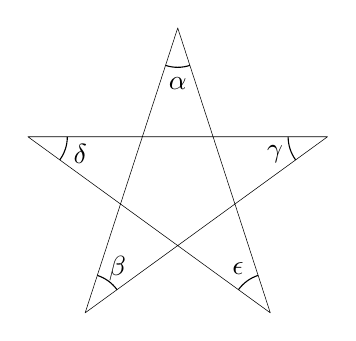
\begin{tikzpicture}[x=1cm,y=1cm]

        \foreach \an\letter in {90/A,162/D,234/B,306/E,378/C}
            { \tkzDefPoint(\an:2){\letter}}
        \tkzDrawPolygon(A,B,C,D,E)
        % \tkzDrawPoints(A,B,C,D,E)

        \tkzMarkAngle[size=0.5,mark=none](B,A,E)
        \tkzLabelAngle[pos=0.7](B,A,E){$\alpha$}
        \tkzMarkAngle[size=0.5,mark=none](C,B,A)
        \tkzLabelAngle[pos=0.7](C,B,A){$\beta$}
        \tkzMarkAngle[size=0.5,mark=none](D,C,B)
        \tkzLabelAngle[pos=0.7](D,C,B){$\gamma$}
        \tkzMarkAngle[size=0.5,mark=none](E,D,C)
        \tkzLabelAngle[pos=0.7](E,D,C){$\delta$}
        \tkzMarkAngle[size=0.5,mark=none](A,E,D)
        \tkzLabelAngle[pos=0.7](A,E,D){$\epsilon$}
    \end{tikzpicture}

    \caption{The aforementioned pentagon whose sum of angles is sought after.}
\end{figure}

\solution

Let's begin by imagining the angles created by the points of intersection of our star's sides
and the inner pentagon formed by these points of intersection.
We will call these angles $a_1$ and $a_2$ for $a$ through $e$,
with the first angles defined as the angles of the interior pentagon and the second angles defined as the exterior angles.

We know that a pair of angles, $a_1$ and $a_2$, will equal $180^\circ$, since they lie on a line, making a straight angle.
The sum of all angles $a_1$-$e_1$ and $a_2$-$e_2$ will therefore equal $540^\circ$.

Um and then do some more stuff\dots
Sorry I'm too lazy.

\subsection{
    Find the sum of angles on the following star-like shape.
}
Given the following modified star-like shape with vertices $A, B, C, D, E, F,$ and $G$,
determine the sum of interior angles $a, b, c, d, e, f,$ and $g$ equal to.

\begin{figure}[h]\label{starB}
    \centering
    \begin{tikzpicture}

        % \foreach \an\letter in {90/A,234/B,306/G,378/C}
        %     { \tkzDefPoint(\an:2){\letter}}
        % \foreach \i in {0..3}

        \def\rot{180}

        \tkzDefPoint(-72+\rot:2){A}
        \tkzDefPoint(-144+\rot:2){C}
        \tkzDefPoint(-216+\rot:2){G}
        \tkzDefPoint(-288+\rot:2){B}

        \tkzDefPoint(-18+\rot:1.6){D}
        \tkzDefPoint(0+\rot:2){E}
        \tkzDefPoint(18+\rot:1.6){F}

        % \tkzDefPoint(162-15:1.8){D}
        % \tkzDefPoint(162:2.2){E}
        % \tkzDefPoint(162+15:1.8){F}

        \tkzDrawPolygon(A,B,C,D,E,F,G)
        \tkzLabelPoints[above](A,D)
        % \tkzLabelPoints[above left](D)
        \tkzLabelPoints[left](E)
        % \tkzLabelPoints[below left](F)
        \tkzLabelPoints[below](B,F)
        \tkzLabelPoints[below right](G)
        \tkzLabelPoints[above right](C)
        % \tkzLabelPoints[](A,B,C,D,E,F,G)
    \end{tikzpicture}

    \caption{The shape whose sum of angles is sought after.}
\end{figure}

\solution

Let's consider the triangle formed by $B$, $C$ and the intersection of $\overline{AB}$ and $\overline{CD}$.
The interior angle formed by the aforementioned angle, which we'l call $\alpha$, is equal to $180^\circ - b - c$.
There's another similar triangle formed by the the vertices $A$, $G$ and another intersection, whose angle we'l call $\beta$.



\end{document}